\documentclass[a4paper, 11pt, twocolumn]{article}

%Handige usepackages voor essays
%\usepackage[protrusion=true,expansion=true]{microtype} % Better typography
%\usepackage{graphicx} % Required for including pictures
%\usepackage{wrapfig} % Allows in-line images
%\usepackage{mathpazo} % Use the Palatino font
%\usepackage[T1]{fontenc} % Required for accented characters
%\linespread{1.05} % Change line spacing here, Palatino benefits from a slight increase by default

%Handige usepackages voor essays
%\usepackage[protrusion=true,expansion=true]{microtype}
%\usepackage{microtype}
\usepackage{graphicx} % Required for including pictures
\usepackage{wrapfig} % Allows in-line images
%\usepackage{mathpazo} % Use the Palatino font
%\usepackage[T1]{fontenc} % Required for accented characters
%\linespread{1.05} % Change line spacing here, Palatino benefits from a slight increase by default

%Standaard usepackages
\usepackage{pdfsync}
\usepackage[english]{babel}
\usepackage{fullpage}
\usepackage{amsmath}
\usepackage[table]{xcolor}
\usepackage{caption}
\usepackage{subcaption}
\usepackage{float}
\usepackage{verbatim}
\usepackage{eso-pic}
\usepackage[toc,page]{appendix}
\usepackage[linkbordercolor={white}]{hyperref}
\usepackage{nameref}
\usepackage{listings}
\usepackage{filehook}
\AtEndOfIncludes{%
  \global\let\savedclearpage\clearpage
  \global\let\clearpage\relax
}
\AfterIncludes{%
  \global\let\clearpage\savedclearpage
}
\makeatletter
\renewcommand{\@listI}{\itemsep=0pt} % Reduce the space between items in the itemize and enumerate environments and the bibliography

\renewcommand{\maketitle}{ % Customize the title - do not edit title and author name here, see the TITLE block below
\begin{flushright} % Right align
{\LARGE\@title} % Increase the font size of the title

\vspace{50pt} % Some vertical space between the title and author name

{\large\@author} % Author name 1
\\\@date % Date

\vspace{40pt} % Some vertical space between the author block and abstract
\end{flushright}
}

%----------------------------------------------------------------------------------------
%	TITLE
%----------------------------------------------------------------------------------------

\title{\textbf{Hardware Implementations of Evolvable Systems}\\ % Title
A critical analysis of autonomic systems with self-properties on reconfigurable architectures } % Subtitle

\author{\textsc{Imara Speek \\ 
Aimee Ferouge} % Author
\\{\textit{Delft University of Technology}}} % Institution

\date{\today} % Date

%----------------------------------------------------------------------------------------

\begin{document}

\twocolumn[
	\begin{@twocolumnfalse}
	\maketitle
	\begin{abstract}
	%----------------------------------------------------------------------------------------
	%	ABSTRACT AND KEYWORDS
	%----------------------------------------------------------------------------------------
	%\renewcommand{\abstractname}{Summary} % Uncomment to change the name of the abstract to something else

Reconfigurable hardware is becoming increasingly more important in in SoC design as it allows efficient hardware acceleration and virtually unlimited adaptability. With the increase of complex,  heterogeneous, multi-core and many-core processors system complexity is skyrocketing. Self-aware adaptive computing systems are capable of adapting their behavior in dynamic environments at run-time to accomplish given goals. This capability on reconfigurable hardware allows for self-adapting and self-optimization during run-time. The increasing presence of heterogeneous architectures such as FPGAs that utilize these techniques make the hardware domain shift more and more into the software domain. 

In this paper we will propose a co-design hardware implementation of evolvable systems that blends the power of flexible software techniques such as monitoring, decision making and self-adaptation with the speed of hardware. The proposed system is composed of a 2D systolic array of processing elements and utilizes partial dynamic reconfiguration in combination with self-properties techniques. 

	\end{abstract}

	\hspace*{3,6mm}\textit{Keywords:} self-aware , computing systems, reconfigurable, autonomic, evolvable % Keywords
		
	\vspace{30pt} % Some vertical space between the abstract and first section
	\end{@twocolumnfalse}
]

%----------------------------------------------------------------------------------------
%	ESSAY BODY
%----------------------------------------------------------------------------------------
\emph{Iets vertellen over dat programmers alleen maar een goal in hoeven te voeren}

% Introduction

\section*{Introduction}

*Introduction* \cite{fpga} blabla \cite{why}

%prior knowledge
\section{Fundamental knowledge}
\label{sec:fundamental}
In this section an introduction to the fundamental terms used in this paper is given. These terms concern prior knowledge required when working with autonomic or evolvable systems and their implementations in hardware. 

Computing system containing \emph{self-properties} are capable of adapting their behavior and resources thousands of times based on changing environmental conditions and demands \cite{selfaware}. This allows them to automatically accomplish their goals in the best way possible. This behavior is achieved through \emph{self-monitoring} which recognizes changes in its internal state that may require a modification, called \emph{self-adjusting}. \emph{Self-healing} concerns effective recovery under fault condition, \emph{self-optimization} invokes optimizing operation in proactive and reactive manners and \emph{self-configuring} concerns automatically installing, configuring and integrating new components seamlessly into the system to meet stated goals \cite{autocom}. 

%\subsection{Evolvable systems}
% what is evolvable
\emph{Evolvable systems} exploit self-adaptive, self-configuring and self-optimizing techniques and are capable of changing their operations to meet the given performance goals by modifying either the underlying heterogeneous architecture, the operating system and the self-adaptive applications. \cite{evolvable}
%Meeting efficiency and accuracy constraints is getting more and more difficult , mainly because of the exponential increase of interactions among systems and the environments in which the systems are required to work. 
%The operating systems chooses at run-time among a set of possible implementations according %to the criteria. This decision is based on the Observe-decide-act. The need for this dynamic %choice between available implementations is give by the fact that the system is live and %lives in an unpredictable environment. \cite{selfaware}

%e explanation of autonomic 
\emph{Autonomic systems} are inpired by the human body's nervous system and contains all self-properties: \emph{self-managing, self-protecting, self-healing} and \emph{self-optimizing} \cite{autonomic}. 

Autonomic and evolvable systems have the need for heterogeneous underlying architectures, which can be provided by using Field Programmable Gate Arrays (FPGAs).These can be configured to fullfil a desired functionality by using one or more bitstreams. These bitstreams are binary files in which FPGA specific configuration information is stored and these are to be copied along with the proper commands on to the configuration SRAM cells, or the configuration memory \cite{reconfigurable}. 
% Discussion of the papers

\section{Discussion of the Different Papers}
\label{sec:discussion}

\emph{[introduction to discussions and seperation of the topics, maybe seperate hardware from software solution from these papers?]
[Give some small introduction to each paper in 3 sentences and then maximum of 15 for every paper]}
\\
\\
Considerable research has already been done in order to efficiently accelerate hardware while still maintaining virtually unlimited adaptability. 
Software techniques in autonomic computing systems such as hot-swapping and data clustering are discussed in \cite{survey}. 
These self-aware systems can adapt their behavior on FPGA-based system as discussed in \cite{selfaware}.
Other approaches start with a FPGA-based architecture with a reconfigurable core \cite{drp},  added programming schemes and new cell structures \cite{virtex4}, \cite{erlangen} or even bio-inspired hardware using the POE-model \cite{poe}.
More recent papers put effort a combined approach by either implementing autonomic systems on reconfigurable architectures \cite{reconfigurable} or creating evolvable systems via self-aware applications \cite{evolvable}.

%% -- Software based papers --------------------------
\subsection{Software based flexible approaches}
\label{sec:software}

%%Survey of Frameworks, Architectures and Techniques in Autonomic Computing

Self-configuration is the ability of the system to perform configurations according to the pre-defined high level policies and seamlessly adapt to change caused by automatic configurations. Self-optimization is the ability of the system to continuously monitor and control resources to improve performance and efficiency. Self-healing is the ability of the system to automatically detect, diagnose and repair faults. Self-protection is the ability of the system to pro-actively identify and protect itself from malicious attacks or cascading failures that are not corrected by self-healing measures.

This paper presents a wide variety of techniques in autonomic computing. Hot-swapping is a technique to inject monitoring and diagnostic code into live code using inter-positioning and replacement. Data clustering is an unsupervised learning algorithm, used to identify configuration classes and determines the degree of similarity between clusters using convex average metric.

				% April, 2009, maybe use this only for prior knowledge
% Software based approaches
The \emph{Heartbeats application} is a monitoring application which makes it possible to assert performance goals as heart-rate windows delimited by a minimum and maximum performance, or \emph{heart-rate} \cite{evolvable}. The Heartbeats API is made of small straightforward functions and allows declaring performance goals. Software components first have to register, specifying parameters such as minimum and maxmim heart-reate, size of the windows of observation and history buffers \cite{selfaware}. The application then updates the progress of the execution calling the function that signifies a heartbeat \cite{evolvable}.

%[SMARTLOCKS PAPER] presents a combination of the Heartbeats application in cooperating with other frameworks. Smartlocks is a spinlock library that will adapt its internal implementations based on defined goals during run-time using heurstics as discussed in subsection \ref{sec:decisions} and machine learning. 

\cite{reconfigurable} dscusses using adaptive programming in situations where input changes lead to relatively small output changes. They present a hardwar/software codesign paradigm that develops a new performance model and associated evaluation metrics to differentiate between various levels of performance across different portions of software modules. Incoorporating this into a codesign environment increases the flexibility of the system. 
%distributed self trained algorithms, machine learning, heartbeats application
%adaptive programming

%% -- Hardware based papers --------------------------
\subsection{Hardware based fast approaches}
\label{sec:hardware}

%% A Phylogenetic, Ontogenetic, and Epigenetic View of Bio-Inspired Hardware Systems

As a final category of evolvable systems, inspired by life on Earth and the natural processes of living organisms, \emph{bio-inspired} hardware systems have evolved. \cite{poe} introduces the POE model, that classifies bio-inspired systems according to three axes:
\begin{itemize}
	\item Phylogeny, where evolvable hardware can be found.
	\item Ontogeny, where systems have the ability to self-repair as the main goal of ontogeny is (cell) growth or construction.
	\item Epigenesis, which is more software-based.
\end{itemize}

By looking at these biological phenomena, researchers can be inspired when developing evolvable hardware systems.					% August, 2002
% The Erlangen Slot Machine: A Dynamically Reconfigurable FPGA-based Computer
\label{sec:erlangen}
FPGAs are commonly used device for implementing the reconfigurable architecture of evolvable systems, especially Virtex FPGAs produced by Xilinx. The \emph{Erlangen Slot Machine (ESM)} from \cite{erlangen} tackles the three major limitations of the Virtex-II FPGA. A pipelined data flow architecture has been used, replacing the finite state machine by a MicroBlaze microcontroller and employing a data crossbar between plug-ins. The ESM has proven to be a valid alternative to the Virtex FPGAs, providing a new architecture to overcome current physical shortcomings of the reconfigurable FPGAs, as well as a new inter-module communication concept and an intelligent module reconfiguration management. 
			% April, 2007
% A Direct Bitstream Manipulation Approach for Virtex4-based Evolvable Systems

In \cite{virtex4} a Virtex4 FPGA implementation is introduced for evolvable systems. Other then earlier versions of Virtex (e.g. the Virtex-II Pro), Virtex4 devices enable two-dimensional dynamic reconfiguration, a feature which considerably reduces the reconfiguration time an thus the evoltuion time (\cite{virtex4}). By using both VRCs (Virtual Reconfigurable Circuits) and direct bitstream manipulation, this new architecture eliminates the biggest limitation of Virtex FPGAs, which is an almost unknown and undocumented bitstream data format and an unsafe configuration schema. 

This Virtex4-based device, which takes advantage of 2D reconfiguration capabilities and direct manipulation of the bitstreams is the first one of its kind and will be discussed later.				% May, 2010
% A Fast Reconfigurable 2D HW Core Archtiecture on FPGAs for Evolvable Self-Adaptive Systms

Another Virtex-4 based architecture introduced in \cite{dpr} also applies the 2D reconfiguration core. Rather than direct bitstream manipulation, a \emph{dynamically partial reconfiguration (DPR)} control engine has been integrated. As a result, the processing elements (PEs) of the reconfigurable core are structured as a 2D systolic array, known for its high performance and restrained use of resources. The reconfiguration engine has been optimized by applying three enhancements that will be discussed in \ref{sec:dpr}.					% June, 2011

%% -- Combinations based papers ----------------------
\subsection{Co-design based systems}
\label{sec:codesign}

% From reconfigurable architectures to self-adaptive autonomic systems 
\cite{reconfigurable} proposes the harvesting of the full potential of dynamic reconfiguration by carefull evaluating the overhead of reconfiguration in hardware-software interfacing. To overcome the limits introduced by increasing complexity and the workloads to main complex infrastructues they propose to adopt a codesigned self-adaptive and autonomic computing system. 
%A full \emph{bitstream} configures the whole configuration memory statically at the beginning of the execution of a system, while partial bitstreams are used for reconfiguration to confirgure merely portions of the device. 

\emph{Partial dynamic reconfiguration (PRD)} is a key feature that makes FPGAs unique. PDR addresses the lack of resources to implement an application and its adaptability needs. Reconfigurable hardware taking advantage of partial dynamic reconfiguration is the perfect trade-off between the speed of HW and the flexibility of SW. \cite{reconfigurable} present an evaluation system, implemented on the Xilinx Virtex-II Pro VP30 on an architecture of two reconfigurable cores. Running an extended version of Linux, the cores can be partial dynamically reconfigured. They compare the performance of three different impementations of a popular encryption algorithm (advanced encryption standard): a reconfigurable IP-core that is configured at runtime (FPGA-RHW), a cached hardware IP-core that is ready to use (FPGA-CHW) and a software implementation (SW) as can be seen in figure \ref{fig:reconfig}. 
% -- reconfig, cached & software ---------------------------
\begin{figure}[htb]%
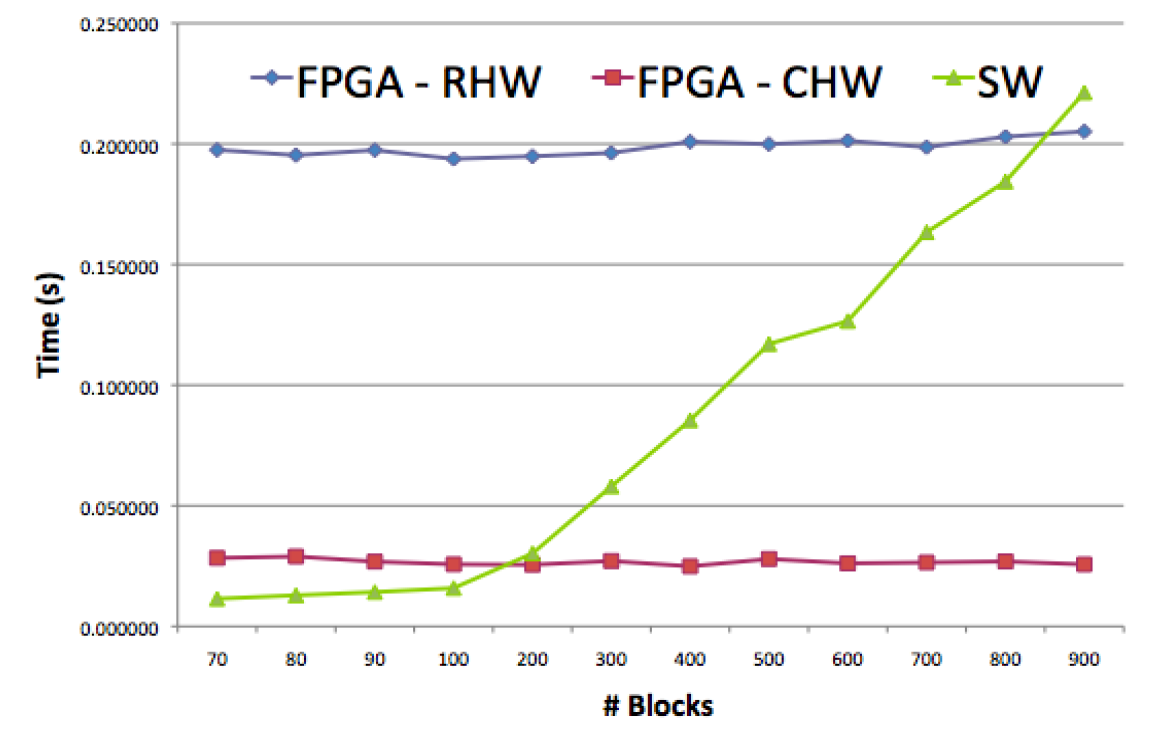
\includegraphics[width=\columnwidth]{Pictures/reconfig.png}%
\caption{Execution time of the implementations of the AES algorithm as seen in \cite{reconfigurable}}%
\label{fig:reconfig}%
\end{figure} 
Figure \ref{fig:reconfig} displays the overhead introduced by reconfiguration. Even though this data was captured in a static analysis, it displays that reconfiguration may dominate the execution. This shows the need for a efficient and fast decision engine, as reconfiguration seems to be only valid in systems of larger than 900 processed blocks. 
%
%However, an important problem often neglected is the time overhead the reconfiguration process introduces and the two-dimensional partitioning strategy reconfigurable devices need: spatial and temporal. \cite{reconfigurable} presents the urge to carefully evaluate the overhead created as a negative impact of reconfiguration latency which is not always discussed in present papers. 
% Evolvable systems on reconfigurable architecture via self-aware adaptive applications. ++
In \cite{evolvable} an evolvable system running self-adaptive application on top of a heterogeneous systems is proposed. 
The operating system running on top is responsible for providing the self-* proporties and runs this on a general purpose processor and a reconfigurable device 

In \cite{evolvable}, the underlying hardware architecture is made up of  static area and a dynamic area. The reconfigurable device can be configured to implement different functionality through dynamic reconfiguration support provided by the operating system. This is provided through standard libraries and the OS implements parts of the loop. The OS is therefor capable of choosing at run-time the best implementation for the required functionality among the available.
The switchable units in the hot-swap method in \cite{evolvable} are identified as the libraries that export an implementation of a certain functionality. 
The self-adaptive library or Dynamic-link library(DLL) and the software implementation library target the reconfigurable FPGA and multicore respectively. 


% Comparison of the techniques presented
\section{Analysis of techniques}
\label{sec:technique}
Reconfiguration capabilities and hardware-software codesign techniques are elements of a complex scenario. This section will discuss and analyze these capabilities and techniques seperately. To create such a self-adaptive autonomic system, the system has to be self-aware, able to make decisions, self-adapting and the hardware has to support a certain amount of reconfiguration. In section \ref{sec:proposition} the overall best combination will be presented, utlizing the flexibility of software and the speed of hardware.

%-----------------------------------------------------------------------------------------

\subsection{Monitoring techniques}
\label{sec:selfawareness}
The heartbeats application as discussed in section \cite{sec:selfaware} is a technique used for monitoring. A framework like this is particularly convenient because it allows to automatically update all information about the global heart-rate which is then made available to external observers, such as decision making applcations. However it introduces an average overhead of 3,52\% due to system calls in order to initialize its data structures and updating the global heart rate \cite{selfaware}.
\subsection{Decision making techniques}
\label{sec:decisions}

* present heuristics, best algorithm etc *
\subsection{Self-adapting techniques}
\label{sec:selfadapting}

A self-aware adaptive computing system is an active system where the hardware, the applications and the operating system have to be seen as an unique entity that can autonomously adapt itself to achieve the best performance. \cite{selfaware} presents a general overview of the hardware and software architecture components of a self-aware computing system as can be seen in figure \ref{fig:selfaware}. Cognitive hardware mechanisms available in the underlying hardware \emph{observe} and \emph{affect} the exectution. 

% -- Plaatje self-aware hardware and software architecture---------------------------
\begin{figure}[htb]%
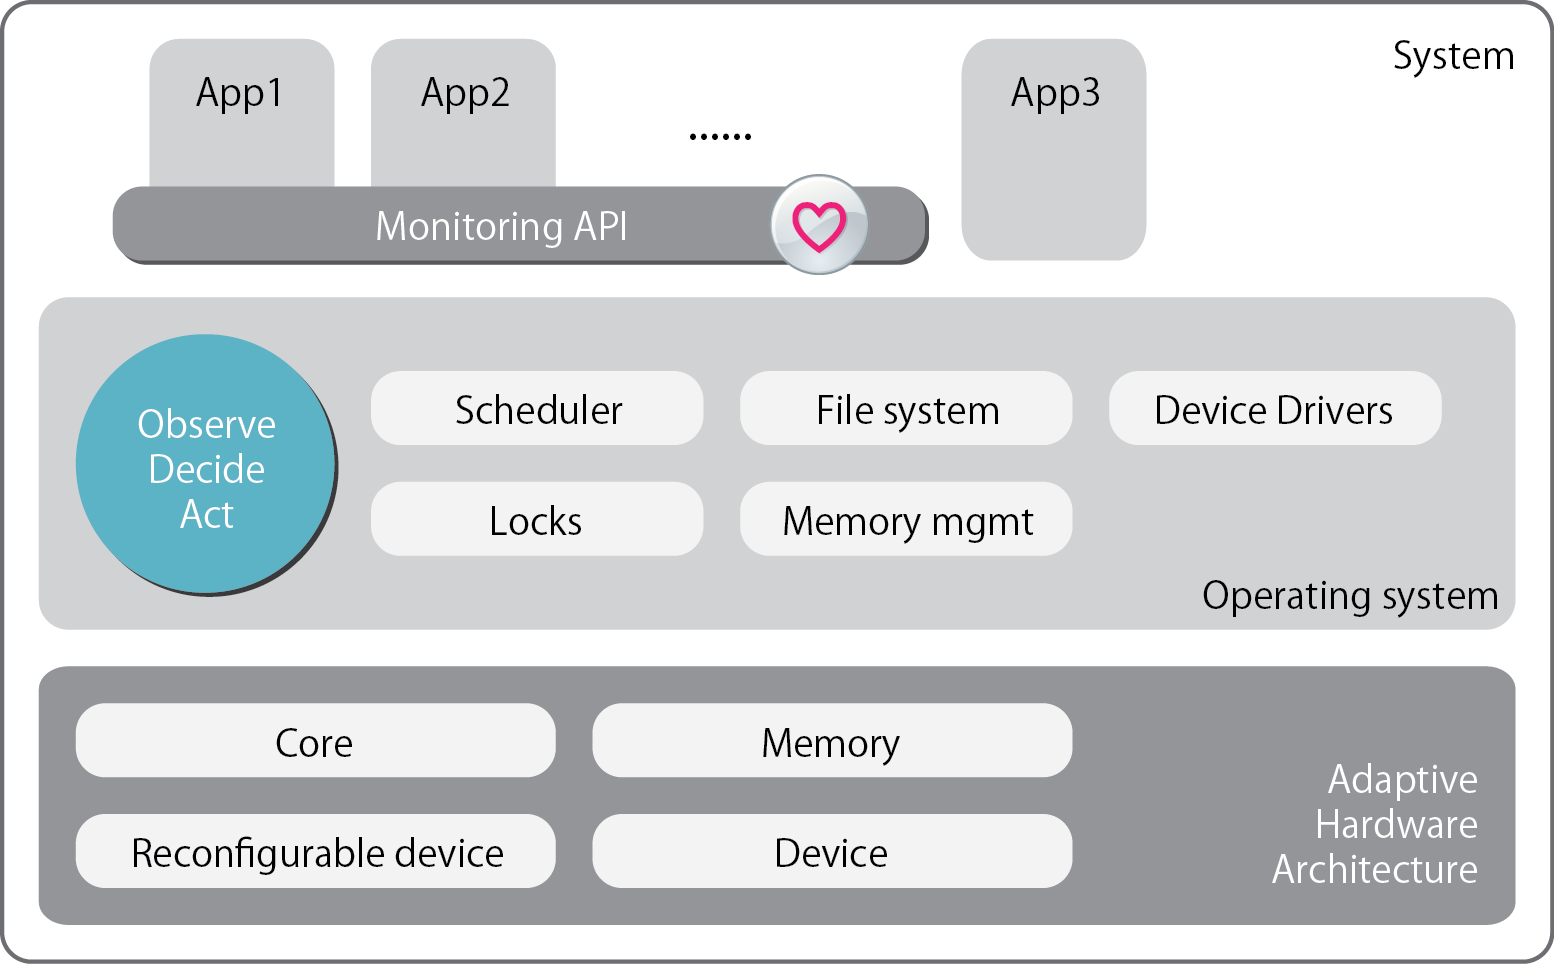
\includegraphics[width=\columnwidth]{Pictures/self-aware.PNG}%
\caption{Overview of the proposed self-aware adaptive FPGA-based computing system presented in \cite{selfaware}}%
\label{fig:selfaware}%
\end{figure}
%------------------------------------------------------------------------------------------------
A fundamental part of a self-aware adaptive computing system is the ability to switch between implementations of the same functionality while the system is running. A control system has to be developed as an actuator in the oberserve-decide-act loop. The \emph{hot-swap mechanism} is a popular tool to inplement self-configuration and self-optimization. Although it provides the ability of switching among different implementations of the same functionality in a transparent fashion, state quiescence and state translation are two big issues when using this mechanism and need a framework solution to be reliable. 

Other works present \emph{Partial Dynamic Reconfiguration (PDR)} \cite{reconfigurable} to reduce the amount of overhead introduced by reconfiguration. Hardware portions can adapt over time to cope with new requirements creating an adaptive system. If the application can be partitioned into different phases, PDR can configure the modules one after another to keep area requirements lower than having all functionalities loaded at the same time. PDR can thus be seen as a trade-off between the speed of hardware and the flexibility of software.  
% Discussion of different hardware techniques
\subsubsection{Virtex FPGA with a Two-Dimensional Reconfiguration Core}
\label{sec:fpga}
On Virtex-4 FPGAs, two-dimensional dynamic reconfiguration as seen in figure \ref{fig:2d} is supported. 2D Reconfiguration enables reconfiguring device portions whose height is not constrained to be the device height. This architecture of the reconfiguration core (RC) speeds up the reconfiguration time and thus the evolution time. The RC can also deploy more candidate solutions as discussed in \cite{virtex4}, these arrays of bidimensional cell can be seen in figure \ref{fig:candidate}. An alternative for candidate solutions is a mesh-type systolic array of parallel processing elements (PEs) from \cite{dpr}, also following a 2D architecture for the RC. A major feature is the possibility to change the functionality of the PEs by means of Dynamic and Partial Reconfiguration (DPR). This gives the system the capability to adapt. The outputs of the PEs (east and south side) are connected to the close neighbour's input (west and north side), such that only the lowest and right-most PE has to be read for data output. This systolic approach of communication reduces the reconfiguration time and makes the architecture scalable.

One drawback of using Virtex FPGAs are the feed-through signals, mentioned in \cite{erlangen}. Each module must be implemented with all possible feed-through channels needed by other modules. Many channels reserved for a possible feed-through are redundant during run-time when the actual implementation is decided upon. Another drawback is the lack of relocation of modules accessing external pins as these are compiled for fixed locations where a direct signal line to these pins is established. 
% -- Plaatje 2D RC architecture ---------------------------
\begin{figure}[htb]%
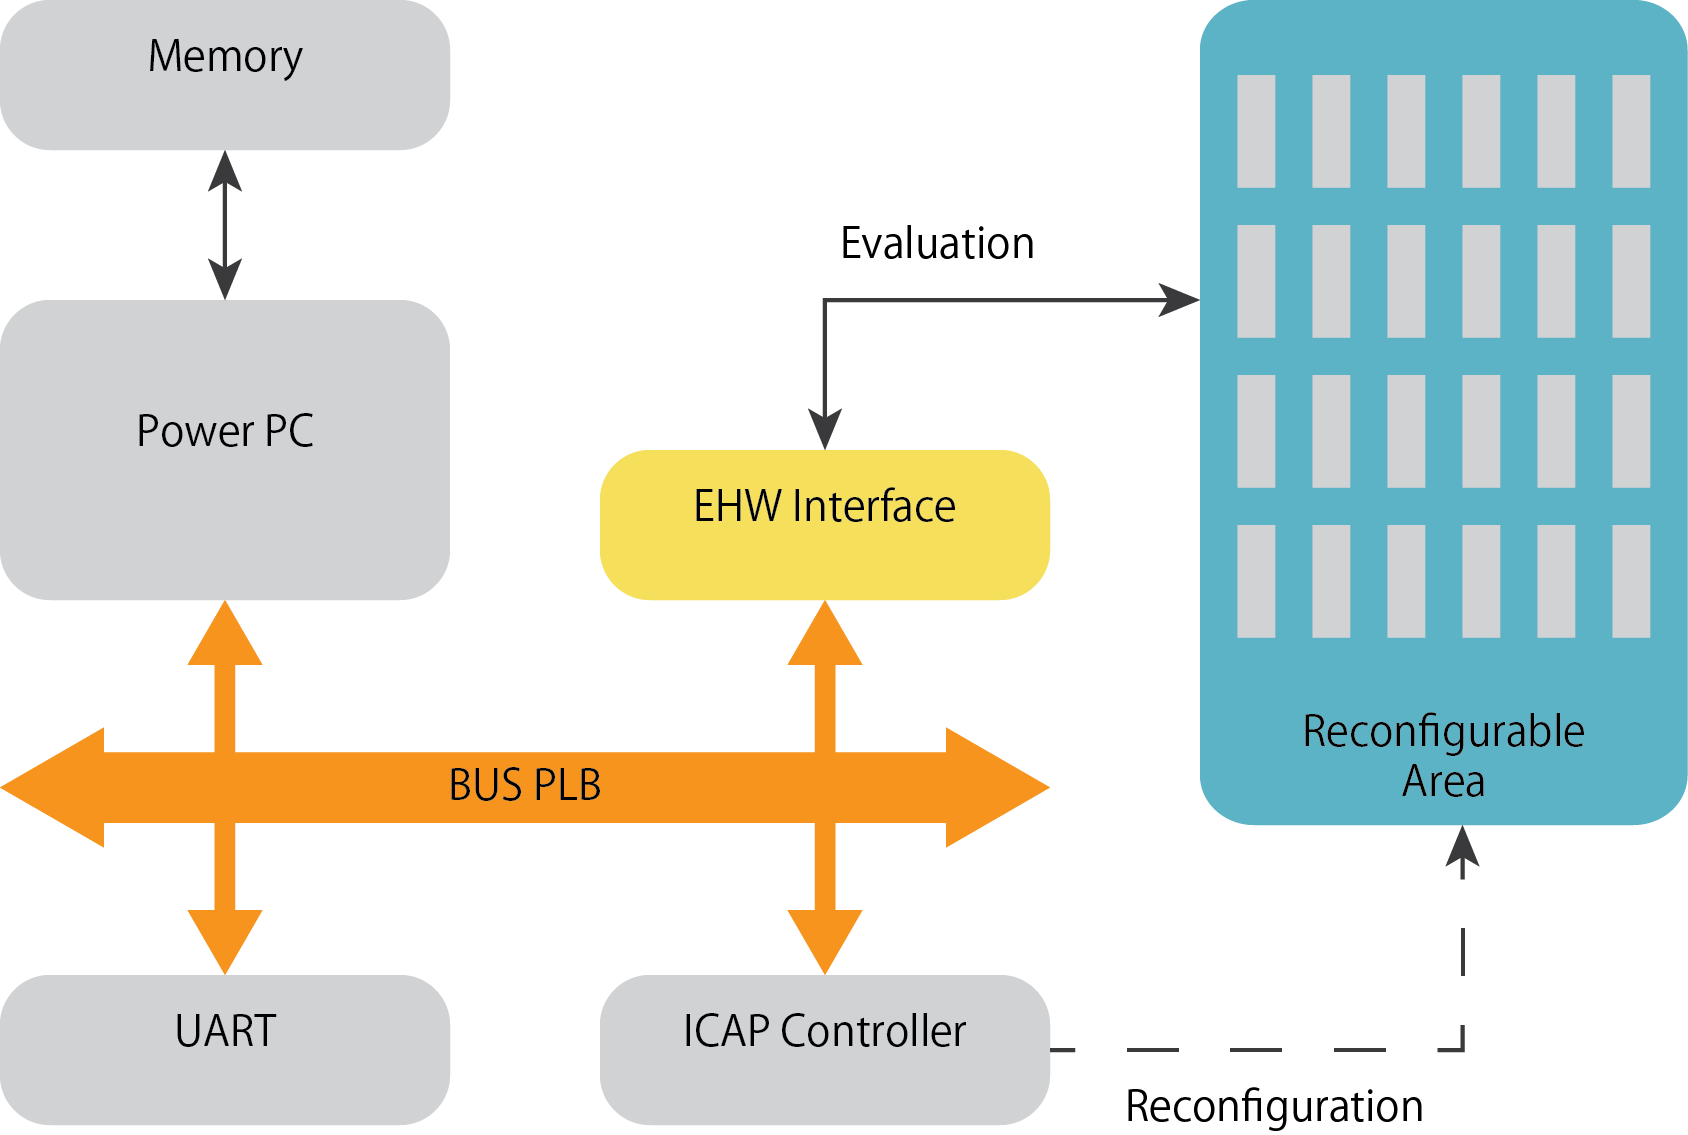
\includegraphics[width=\columnwidth]{Pictures/2D_architecture.png}%
\caption{High-level structure of a Two-Dimensional Architecture depicted in \cite{virtex4}}%
\label{fig:2d}%
\end{figure}

\subsubsection{Candidate Solutions and Direct Bitstream Manipulation}
\label{sec:candidate}
\cite{virtex4} uses safe manipulation \emph{UITLEGGEN WAT SAFE MANIPULATION IS} of the bitstream in a 2D architecture for the RC to overcome the unknown and undocumented bitstream mentioned in \ref{sec:virtex4}. Candidate solutions are used to fill the RC with cells, which have internal flip-flops allowing the evolution of synchronous circuits. This is a common structure for \emph{evolvable hardware (EHW)} systems making use of direct bitstream manipulation \cite{virtex4}. For the cell structure of the candidate solutions the use of \emph{look-up tables} and a \emph{multiplexer} is proposed to provide direct bitstream manipulation. Combined with the 2D-reconfiguration mechanism, the new architecture causes a speed up of 16x factor. For this system, only Virtex-4 or Virtex-5 FPGAs can be used since Virtex-II does not support 2D reconfiguation \cite{virtex4}. \emph{COMPARED TO WHAT??}

% -- Plaatje candidates ---------------------------
\begin{figure}[htb]%
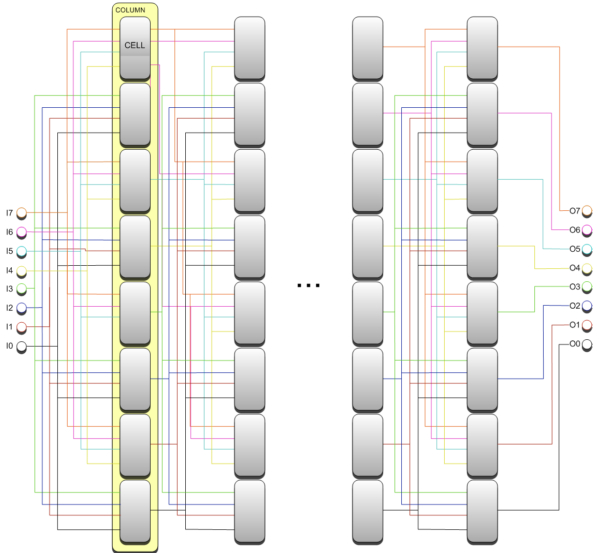
\includegraphics[width=\columnwidth]{Pictures/candidate.png}%
\caption{Internal structure of a Candidate Solution proposed in \cite{virtex4}}%
\label{fig:candidate}%
\end{figure}

\subsubsection{Systolic array of PEs and Optimized DPR}
\label{sec:dpr}
Other than \cite{virtex4}, \cite{dpr} uses a systolic array of PEs. In this approach, each PE is a basic computation unit able to perform a single operation on the data take from their close neighbors. The architecture can be easily extended to any other processing purposes, since new PEs can be added to the library. In addition, PEs included in this library can be reused among applications. As can be seen in fig. \ref{fig:pe}, the size of the implemented structure is 4x4, but it is scalable. This DPR with elements relocation is carried out using a special hardware block, the \emph{reconfiguration engine (RE)}.

\cite{dpr} describes an implementation of this RE. Only the body of the bitstream (cutting of the header and the tail) is stored, the FPGA is overclocked by 2,5x and internal memory is included to avoid pasting the same configuration module in different positions of the architecture. This optimization of DPR recudes the reconfiguration time. Adding the header and the tail of the bitstream at runtime has two additional advantages: it allows having a unique bitstream for each PE that can be configured in any position of the array and reduces the data transference time from the external memory.

% -- Plaatje systolic PE array architecture ---------------------------
\begin{figure}[htb]%
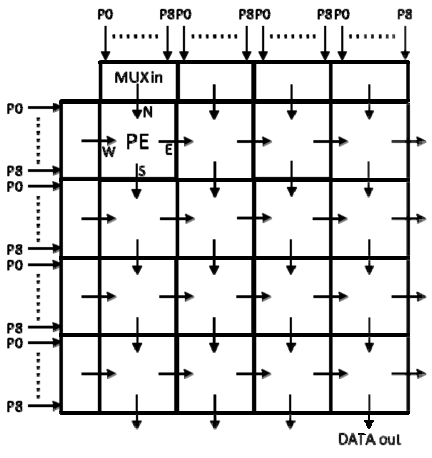
\includegraphics[width=\columnwidth]{Pictures/PE}%
\caption{Systolic array of PEs introduced by \cite{dpr}}%
\label{fig:pe}%
\end{figure}

\subsubsection{Erlangen Slot Machine}
The \emph{Erlangen Slot Machine (ESM)} presented in \cite{erlangen} deals with the three drawbacks of FPGAs mentioned in \ref{sec:fpga}. Fixed pins are spread around the device causing the I/O dilemma, the inter-module dilemma and the local memory dilemma. 

First, the I/O dilemma caused by fixed pins spread around the device is solved by connecting all bottom pins from the FPGA to an interface controller realizing a crossbar, as can be seen in figure \ref{fig:erlangen}. It connects FPGA pins to peripherals automatically based on the slot position of a placed module. This I/O rerouting principle is done without reconfiguration of the crossbar FPGA.

Second, the memory dilemma has been solved. In default Virtex-II FPGAs, a module can only occupy the memory inside its physical slot boundary. Storing data in off-chip memories is therefore the only solution. \emph{IS DIT ECHT WAAR, IS NOGAL EEN STATEMENT} In the \emph{ESM}, six SRAM banks are connected to the FPGA. Since these banks are placed at the opposite side as the crossbar, a module will connect to peripherals from one side, while the other side will be used for temporally storing computational data. In order to use a SRAM bank (called a slot), the module must have at least a width of three micro-slots, in which the total device is divided as can be seen in figure \ref{fig:erlangen}. This organization simplifies relocation, enabling a partially reconfigurable computing system and enables the availability of equal resources for each module.

Finally, the inter-module communication dilemma is dealt with. The ESM uses a combination of bus-macros, shared memory, RMB (Reconfigurable Multiple Bus) and a crossbar to take away the limiting factor for the wide use of partial dynamic reconfiguration (\cite{erlangen}).
% -- Plaatje ESM ---------------------------
\begin{figure}[htb]%
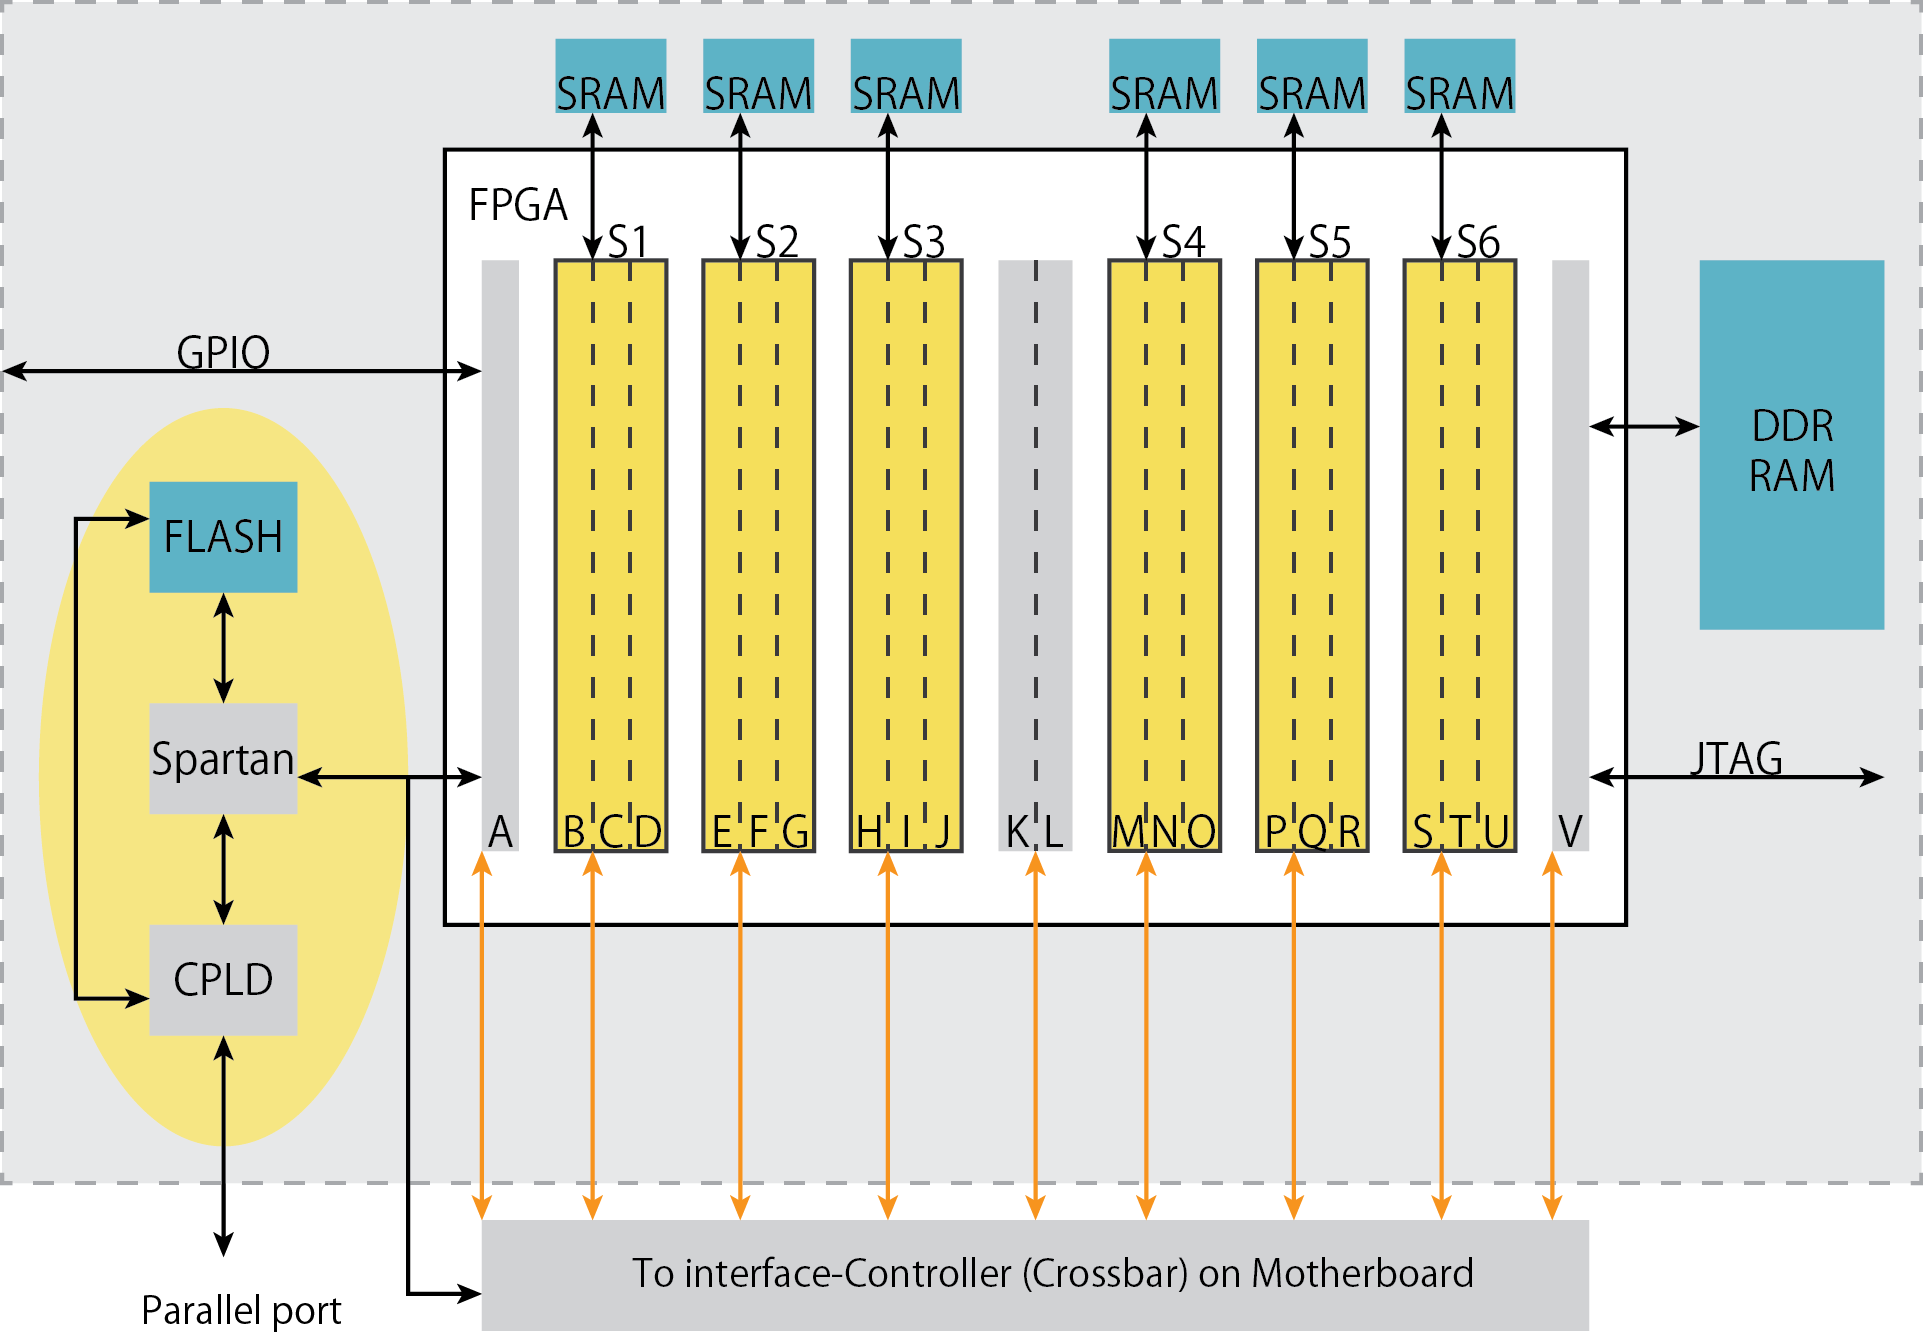
\includegraphics[width=\columnwidth]{Pictures/erlangen}%
\caption{Architecture of the ESM board. Three consecutive micro-slots define a macro-slot, which can access one full external SRAM bank.}%
\label{fig:erlangen}%
\end{figure}


% not important papers
%%Self-managed Systems: An Architectural Challenge

A self-managed software architecture is one in which component automatically configure their interaction in a way that is compatible with an overall architectural specification to achieve the goals of the system. Dynamic change which occurs while the system is operational, is far more demanding and requires the system to evolve dynamically and that adaption occurs at run-time. There is a community called SEAMS (Software engineering for adaptive and self-managing systems).

They focus on the use of ADLs for software design and implementation from components, including limited language support for dynamic change, a general model for dynamic change and evolution, associated analysis techniques and initial steps towards self-management.

The three-layer Gat model is presented. The bottom control layer consists of sensors, actuators and control loops and includes facilities to report the status to the middle layer. The change management layer, or middle layer reacts to state changes accordingly and can introduce new components. The upper goal layer consists of time consuming computations such as planning. They propose a component design that implements the set of services that it provides and the set that it may need.

		% May, 2007, not usefull, just for the intro
%% A New Architecture for Trustworthy Autonomic Systems

Validation alone does not always guarantee trustworthiness as each individual decision could be correct, but the overall system might not be consistent or dependable. These aspects should be integrated at architectural level and not be seen as add ons. Autonomic computing is mostly based on the architecture's basic MAPE (monitor, analyze, plan, execute) control loop. Another inspiration for autonomic systems is Intelligent Machine Design (IMD), based on the human autonomic nervous system.

In large systems with a wide behavioral space it is highly complex to determine whether all autonomic decision were in overall interest of the system. There is a vital need to dynamically validate the run-time decisions of the autonomic manager. The higher goal is not to just reach self-management, but to achieve consistency and reliability of results through self-management.

Current research has looked into a fifth state of the self* properties: self-regulation. It tests itself integral in the architectural, however it assumes that the other states perform optimally and they do not ensure trustworthiness. Another believe is that trustworthiness is achieved when keeping an account of its behavior. This requires the user to intervene if necessary. A dead-zone can be introduced to prevent unnecessary inefficient and ineffective control brevity when the system is sufficiently close to its target value.

The proposed trustworthy architecture exists out of  Autonomic Controller, an Validation Check, a Dependability Check and the managed sub-system. The AC doesn't matter about the content of the unit, but only provides an interface to the designers to express rules that govern the goal. The VC is a higher level mechanism that keeps track of the goal. It is important to also consider the possibility of overall inconsistency in the behavior of the system (the AM could erratically be changing its mind, causing oscillation). The DC only allows the AM to change its mind when its necessary and safe to do so.  Dead-zone logic is implemented to account for this, as well as prediction and learning. A system, no matter the context of deployment, is truly trustworthy when its actions are continuously validated to satisfy set requirements.
	% September, 2012


% Proposition of a evolvable system on a reconfigurable architecture

\section{Proposed Adaptive System Design}
\label{sec:proposition}

Given all these techniques, the question rises which of them could become promising when being combined with each other. In this section, a design is being proposed mixing and matching the previous techiques based on their advantages and drawbacks. By doing this, we first look at the hardware implementations, since these are responsible for the physical limitations. Afterwards, several software techniques are considered in order to add the evolvable behaviour to the system.

% --- HW Proposal --------------------------------------

\subsection{Proposed Hardware}
\label{sec:hardware}

The architecture introduced in \cite{PDR} seems the most promising architecture. Whereas \cite{virtex4} is still discovering the two-dimensional reconfigurability using rigid columns with static routing, \cite{PDR} is applying \emph{Partial Dynamically Reconfiguration}, enabling the system to reconfigure certain parts while others keep running their program. Keeping the idea of evolvable systems in mind, this feature enables an \emph{autonomic system} best. Also, the designers have used their one drawback (the addition of an enhanced ICAP) to include two more system improvements concerning the speed up. 

A quantative comparison between all three the hardware implementations will be covered in Section \ref{sec:related}.

% --- SW Proposal --------------------------------------------
\subsection{Proposed Software}
\label{sec:prosoftware}
The evolvable framework co-designed with the proposed hardware has to include a monitoring technique, a decision making engine and an adaptation framwork. The Evolutionary Framework proposed in \cite{PDR} is based on an evolutionary algorithm that uses static input data files as reference for its evolution. This section proposed an adaptable fully autonomous system on top of our heterogeneous architecture. 

The \emph{HeartBeats application} is proposed as the monitoring technique as it enables the system to predefine performance goals and delivers real-time information to the decision engine. This will introduce a moderate overhead by initializing the data structures which will relatively decrease when dealing with larger complex systems. This is acceptable as Section \ref{sec:codesign} displayed that the use of evolvable system only becomes valid when working with these complex systems. This run-time information will support an agile self-aware system. 

The monitoring system will feed the performance information to the decision engine. Inspired by the PDR methods a partial dynamic model is proposed. A combination of an \emph{analytical} and \emph{empirical model} will enhance the initial performance of the system as it has priorly developed knowledge in the analytical model. The empirical model can take over when performance goes out-of -bounds to handle unexpected behavior. 

PDR will reduce the amount of overhead introduced by reconfiguration during self-adapting. However a framework to adapt, or switch between implementations of functionalities still has to be provided. The \emph{Implementation Switch Service} inspired by the \emph{hot-swap mechanism} as proposed in \cite{selfaware} solves the state quiescence and state translation and thus completes the proposed evolvable framework.


% Comparing presented combination with related works and combinated techniques

\section{Related works}
\label{sec:related}

%\emph{a presentation of related combination of techniques presented in previous paper}
%[I think the POE model paper should be mentioned here instead of Discussion, since its not a HW implementation]
%% A Phylogenetic, Ontogenetic, and Epigenetic View of Bio-Inspired Hardware Systems

As a final category of evolvable systems, inspired by life on Earth and the natural processes of living organisms, \emph{bio-inspired} hardware systems have evolved. \cite{poe} introduces the POE model, that classifies bio-inspired systems according to three axes:
\begin{itemize}
	\item Phylogeny, where evolvable hardware can be found.
	\item Ontogeny, where systems have the ability to self-repair as the main goal of ontogeny is (cell) growth or construction.
	\item Epigenesis, which is more software-based.
\end{itemize}

By looking at these biological phenomena, researchers can be inspired when developing evolvable hardware systems.
%
%* present 3 tier architecture of \cite{evolvable} where the observe-decide-act loop resides in the self-adaptive libraries *
%
%The K42 object oriented operating system created by IBM supports online reconfiguration \cite{evolvable}
%
%Smartlocks is a spinlock library that adapts its internal implementation during execution using heuristics and machine learning. It optimizes towards a user-defined goal, programmed using the application heartbeats framework, which may relate to performance, power, problem-specific criteria or combinations. \cite{reconfigurable}
%
%present self-aware adaptive computing system with implementation switch service figure 2

% -- Kwantitatieve analyse technieken ----------------------------------

The software used by the system to evolve certain application is called the Evolutionary Algorithm (EA): a generic population-based metaheuristic optimization algorithm. Candidate solutions play the role of individuals in the population. At every iteration, a new generation of candidate solution is created. For each generation, the genetic algorithm uses the current population to create the children that make up the next generation. The algorithm selects a group of individuals in the current population, called parents, who contribute their genes (the entries of their vectors) to their children. The algorithm usually selects individuals that have better fitness values as parents. 

For performance experiments, \cite{virtex4} uses a standard testbench to prove the EHW systems effectiveness. The system is being requested to evolve a parity generator in order to report the results of the EA. A parity generator checks data to be transmitted for logic '1's.If the number is even, the parity bit is set to '1'. If the number is odd, parity bit is '0'. For executing this task, the average duration of the EA runs is 7,9 seconds for a 5-bit input number (and 76,8 seconds for an 8-bit number). A second experiment concerning the evolution of communication channels causes trouble, since the fine-grained evolution by evolving candidate solutions at low level (using direct bitstream manipulation) is not able to succeed most of the times. A third experiment involves the evolution of a counter. For a 3-bit counter, using low level evolution and six columns of cells, the average evolution time of 2,7 seconds is needed. For a 4-bit counter, however, the system failed almost every time. [add a qualitative value to the numbers of generation]

Although the ESM introduced in \cite{erlangen} sounds promising, the machine is a customized design that has been manufactured only in very small amounts at the University of Erlangen-Nuremberg. In order for this system to become wide-spread, all parts have to become easy to assemble for mass production. Their case study about video and audio streaming started with a data block-oriented reconfiguration manager. Unfortunately, the maximum upload speed of a bitstream to the FPGA was slowed down by factor two, due to the bottleneck of scratch pad-oriented data flow combined with the sequential execution of the instructions. When applying a pipelined data flow architecture as mentioned in \ref{sec:erlangen}, however, additional plug-ins can be added such that the bitstream can be uploaded into the FPGA at the speed of the flash interface. The article concludes with a proposal to add another decompression plug-in in order to further increase the data rate of the bitstreams from 10 MB/s to 50 MB/s, but has no further numbers to quantitavely beat the existing FGPA-based platforms. Maybe this system will have break through in a couple of years.

As for \cite{dpr}, evolution of image noise filters is selected as the proof of concept application. The average evolution time needed to achieve a correct result is 128 seconds, which at first seems hard to compare to the 2,7 seconds of the 3-bit counter mentioned in \cite{virtex4}. However, given the fact that the input image is a 256 x 256 image (with each pixel existing of 8 bits), this result is quite impressive. 

evolution of communication channels
evolution of a counter
evolution of a controller for the inverse pendulum problem


% Conclusion and Future Challenges

\section{Conclusion}
\label{sec:conclusion}
In this paper, a hardware implementation of an evolvable system is proposed. The two-dimensional reconfigurable architecture using systolic arrays of processing elements enabling partial dynamically reconfiguration and its co-designed evolvable framework supporting the HeartBeats monitoring application an empirical model based decision engine and a hot-swap inspired self-adapting framework is based on a critical analysis of current research in autonomic and evolvable systems on heterogeneous architectures. 

The proposed design was derived after discussing current research in the field of evolvable systems and heterogeneous architectures and extracting the techniques that are utilized. Although a deeper understanding is given into the world of autonomic systems, future work would have to invest in providing an analytical understanding. Proposed future work would be running benchmarks for these systems so the techniques that were used can be compared seperately and in co-design. 

This paper provides a deeper understanding into co-design of hardware and software that is becoming increasingly important considering the current increase in system complexity and size.

%----------------------------------------------------------------------------------------
%	BIBLIOGRAPHY
%----------------------------------------------------------------------------------------

\bibliographystyle{plain}

\bibliography{References}

%----------------------------------------------------------------------------------------

\end{document}